\section{Performance Analysis}
First, we begin with a performance analysis of EMBERS, from both a quantitative
point of view with respect to the GSR and with respect to end-user (analyst) goals.
\subsection{Quantitative Metrics}
\begin{figure}
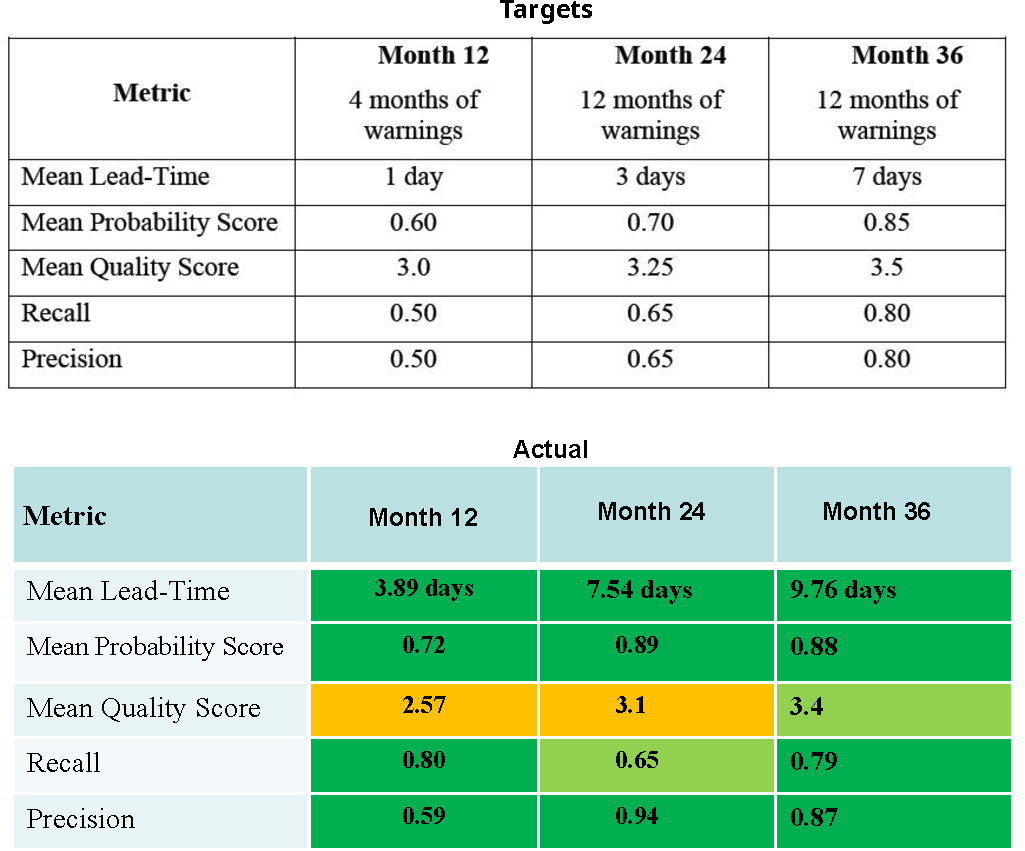
\includegraphics[width=0.8\columnwidth]{figures/cu/performance_tb1}
\caption{IARPA OSI targets and results achieved by EMBERS}
\label{quant}
\end{figure}
Fig.~\ref{quant} depicts both the targets set by the IARPA OSI program as well as the
actual measures achieved by the EMBERS system. As shown here, the easiest target to achieve
in EMBERS was, surprisingly, the lead time objective. This was feasible due to EMBERS's focus on modeling
both planned and spontaneous events. Planned events are sometimes organized with as many as several weeks
of lead time and thus identifying indicators of organization was instrumental in achieving
lead time objectives. The confidence (mean probability) scores were also achieved by EMBERS and involved
careful calibration of probabilities by taking into account estimates of
model propensities and data source reliabilities. The measure that was most difficult to achieve
was the quality score as it involved a four component additive score and thus tangible improvements in
score required more than incremental improvements in forecasting specific components. Finally, recall
and precision involve a natural underlying trade-off and the deployment of our fusion/suppression
engine provided the ability to balance this trade-off to meet IARPA OSI's objectives.

Apart from comparing mean scores another interesting metric is to see
how many perfect matches (4.0 quality score) is obtained by a
algorithm.Fig.~\ref{fig:perfect_score} shows the number of alerts issued
by EMBERS that matched perfectly to an event in the future on a monthly
basis for 2013.The figure clearly shows that EMBERS makes almost double
the number of fully accurate forecasts as compared to the baserate
model.

% SATHAPPAN INSERT the quant table here.

\subsection{Analyst Evaluation}
In addition to the quantitative measures above, our experience interacting with analysts (across multiple
branches of government) demonstrated
an interesting dichotomy to how analysts use EMBERS alerts. Some analysts preferred to use EMBERS in an
`analytic triage' scenario wherein they could tune EMBERS for high recall so that they would apply their
traditional measures of filtering and analysis to hone in on forecasts of interest. Other analysts
instead viewed EMBERS as a data source and preferred to use it in a high precision mode, e.g., wherein they
were focused on a specific region of the world (e.g., Venezuela) and aimed to investigate a particular
social science hypothesis (e.g., whether disruptions in global oil markets led to civil unrest).
To support this dichotomy of users, we implemented a mechanism wherein in addition to generating alerts, EMBERS
also forecast the expected quality score for each forecast (using machine learning methods trained on
past GSR-alert matches). This expected quality score measure provided a way for analysts to use quality
directly as a way to tune the system to receive greater or fewer
alerts.Figure.~\ref{recallVsQS} shows the trade-off between final quality
score and recall when alerts are suppressed based on expected quality.
As expected we can see that the recall drops and quality increases as the cut-off
threshold for expected quality is increased.


\begin{figure}
\centering
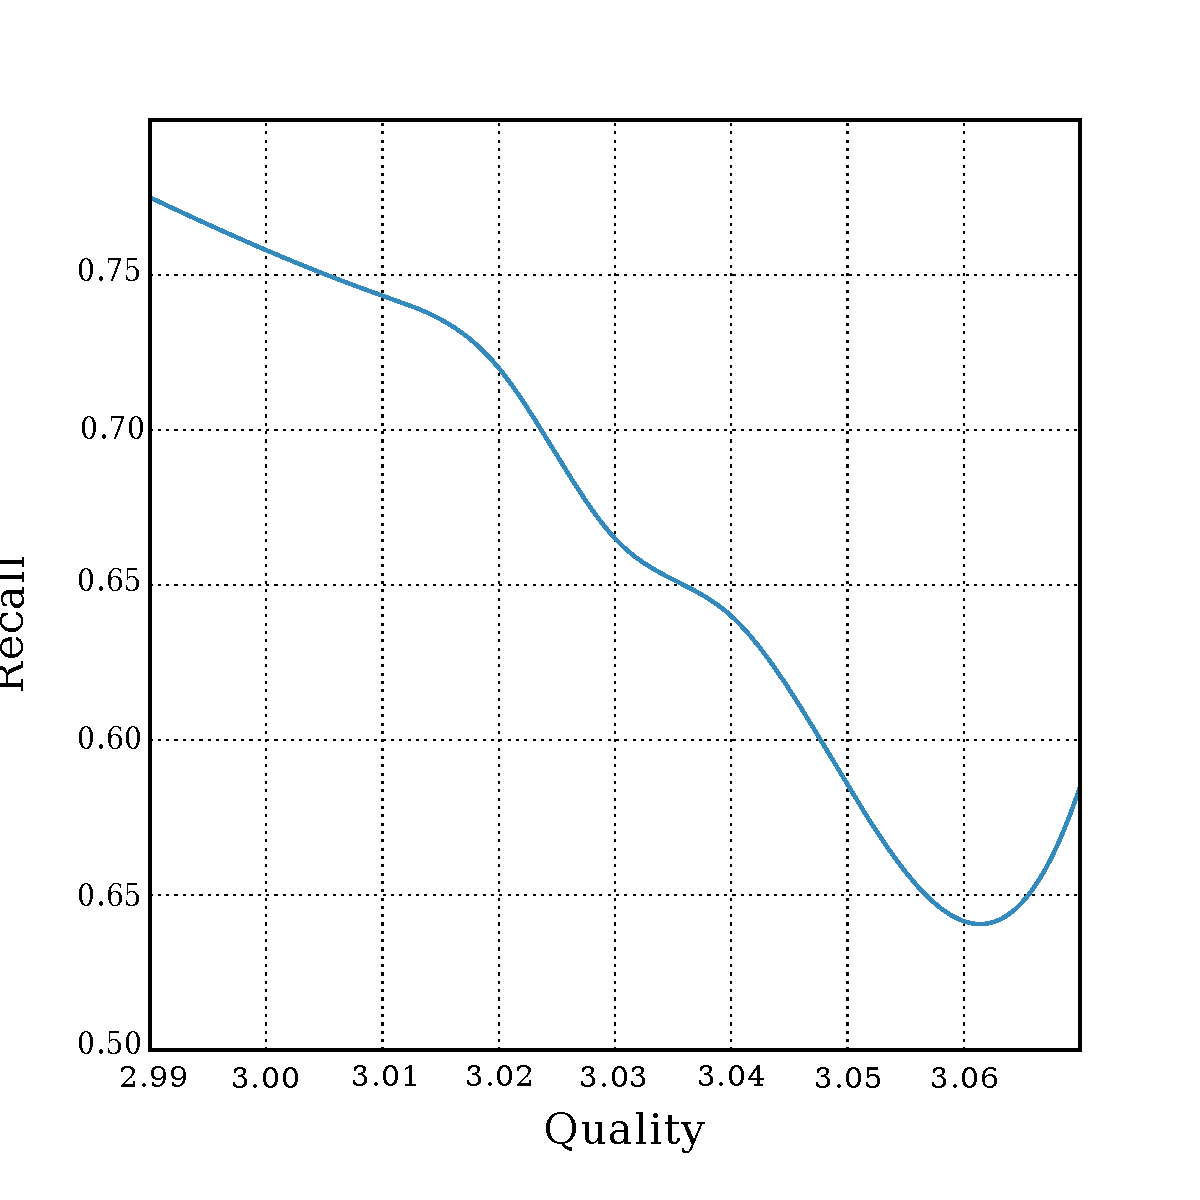
\includegraphics[height=0.2\textheight]{figures/cu/recallVsQS.pdf}
\label{fig:recallvsQS}
\caption{Recall vs Quality Trade-off}
\end{figure}

\narenc{Show forecast with comment describing predicted QS.}
\narenc{Insert quality score tuning curve here.}
\begin{figure}
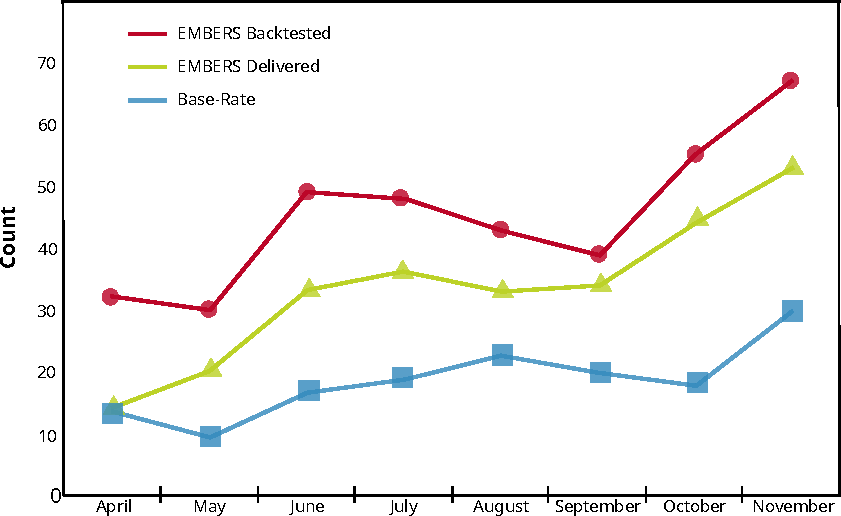
\includegraphics[width=\columnwidth]{figures/cu/perf_figures.pdf}
\caption{Comparison of number of perfect scores(4.0) obtained by EMBERS vs BaseRate per month in 2013.}
\label{fig:perfect_score}
\end{figure}

\narenc{Insert narrative here.}
\begin{figure} %[!t]
    \centering
    \fbox{
\begin{minipage}{\columnwidth}{
EMBERS forecasts that there will be a {\color{red}violent} protest on
{\color{red}February, 18th 2014}
in {\color{red}Caracas}, the {\color{red}capital city of Venezuela}.
We predict that the protest will involve
people working in the {\color{red}business sector}. The protest will be related to
{\color{red}discontent about economic policies}.
\\
There were {\color{blue}5, 5, and 5 other similar
warnings in last 2, 7 and 30 days}, respectively.
\\
The forecast date of the warning falls in {\color{blue}week 7}, which
{\color{blue}may have historical
importance}; this {\color{blue}week is found to be statistically significant}
(pval=0.00461919415894, zscore=2.832, avg. count=57.25, mean=21.569 +/- 12.597)
\\
Audit trail of the warning includes an {\color{blue}article printed 2014-02-17}.
\\
\underline{Major players} involved in the protest include {\color{red}Venezuelan opposition leader, students,
President Nicolas Maduro, and Leopoldo Lopez}.
\\
\underline{Reasons}: Protest {\color{magenta}against rising
inflation and crime}; Protestors want a {\color{magenta}political change}; President Nicolas
Maduro has {\color{magenta} accused US consular officials} and {\color{magenta}right-wing}.
\\
\underline{Protests are characterized by}: Venezuelan opposition leader
spearheaded days of protest and {\color{green}calling for peaceful
demonstration}; Maduro accused official on {\color{red} 2014-12-16}; Protests
have seen {\color{green}several deadly street protests}; Three people were
{\color{green}killed on} {\color{red}2014-02-12}; {\color{green}Demonstrations}
setting days of clashes; {\color{green}supporters to march to}
{\color{red}Interior Ministry} {\color{green}on} {\color{red}2014-02-18}.
}
\end{minipage}
}
    \caption{An example narrative for a EMBERS alert message. Here, color
{\color{red}red} indicates named entities, {\color{green} green} refers to
descriptive protest related keywords. Items in {\color{blue} blue} are historical or
real time statistics and those in {\color{magenta}magenta} refer
to inferred reasons of protest. }
    \label{fig:narrative}
\end{figure}

\narenc{Write explanation of how narrative(Fig.~\ref{fig:narrative}) was come up with.}
